\chapter{PREREQUISITES}

\section{Merkle Trees}
\noindent{
Merkle trees are created by repetitively hashing pairs of nodes until only one hash is left, this hash is better called the Merkle Root or the Root Hash. They are constructed from the bottom, from the hashes of individual transactions called Transaction IDs. Thus every leaf node is a hash of transactional data, and each non-leaf node is a hash of its previous hash. }
\begin{figure}[H]
    \centering
    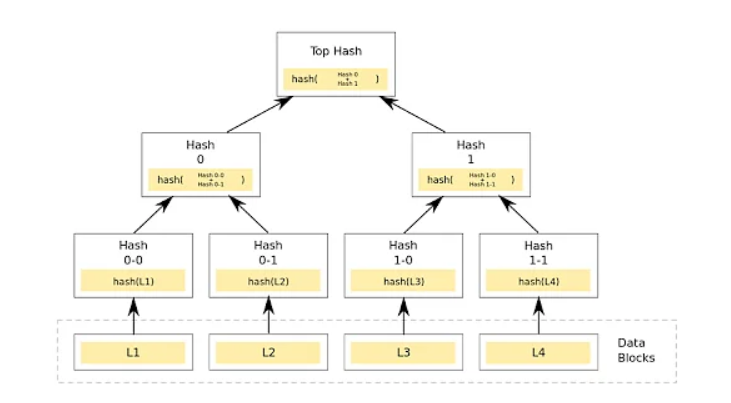
\includegraphics[width=\textwidth]{imgs/merkel_tree.png}
    \caption{Working of Merkle Tree}
    \label{fig:Working of Merkle Tree}
    \end{figure}
    \section{SHA-256}
    \noindent{ 
    SHA 256 is a math process that generates a 256 bit (64 character long) random sequence of letters and numbers (hash) out of any input.Hashing is used to make storing and finding information quicker because hashes are usually shorter and easier to find. The number of possible combinations of letters and numbers produced by SHA 256 exceeds the number grains of sand on Earth! That makes guessing the data hidden within the hash virtually impossible. Hashes cannot be reversed.}    

    \section{Proof Of Work ( POW )}
\noindent{The proof-of-work protocol, Ethash, requires miners to go through an intense race of trial and error to find the nonce for a block. Only blocks with a valid nonce can be added to the chain.\\
When racing to create a block, a miner will repeatedly put a dataset, that you can only get from downloading and running the full chain (as a miner does), through a mathematical function. The dataset gets used to generate a mixHash below a target nonce, as dictated by the block difficulty. The best way to do this is through trial and error.\\
Once generated, this is incredibly easy for other miners and clients to verify. Even if one transaction were to change, the hash would be completely different, signaling fraud.
Hashing makes fraud easy to spot. But proof-of-work as a process is also a big deterrent to attacking the chain\\
The objective of proof-of-work is to extend the chain. The longest chain is most believable as the valid one because it's had the most computational work done. Within Ethereum's PoW system, it's nearly impossible to create new blocks that erase transactions, create fake ones, or maintain a second chain. That's because a malicious miner would need to always solve the block nonce faster than everyone else.}


\section{Proof Of Stake ( POS )}
\noindent{Proof of stake is a type of consensus mechanism used by blockchain networks to achieve distributed consensus.It requires users to stake their ETH to become a validator in the network. Validators are responsible for the same thing as miners in proof-of-work: ordering transactions and creating new blocks so that all nodes can agree on the state of the network.
Proof-of-stake comes with a number of improvements to the proof-of-work system:
better energy efficiency – you don't need to use lots of energy mining blocks
lower barriers to entry, reduced hardware requirements – you don't need elite hardware to stand a chance of creating new blocks
stronger immunity to centralization – proof-of-stake should lead to more nodes in the network
stronger support for shard chains – a key upgrade in scaling the Ethereum network.}
 
\section{Digital signature }
\noindent{It uses public key cryptography to validate and ensure  authenticity and integrity of the signed information. Let’s have a look at how digital signature uses public key cryptography for signing and verification operations.}
\begin{itemize}
\item Authentication: When a verifier validates a digital signature using the sender's public key, he is confident that the signature is of the sender with an associated secret private key.
\item Data Integrity: If an attacker edits the data, the digital signature verification at the receiver end fails. The hash of updated data and the verification algorithm’s result will not match. As a result, the receiver can securely reject the message.
\item Non-repudiation: Because the signature key is known only to the signer, he can create a unique signature on a given data. In the event of a future disagreement, the receiver might offer the data and digital signature to a third party as evidence.
\end{itemize}\


\section{51\% Attack}
\noindent{A 51\% attack refers to an attack on a blockchain by a group of miners controlling more than 50\% of the network's mining hash rate or computing power. The attackers would be able to prevent new transactions from gaining confirmations, allowing them to halt payments between some or all users.}

\section{Blockchain}
\textit{Decentralized.Transparent. Anonymous. Consensus Base. Immutable. Open Source.\\}
\underline{Blockchain Structure}\\

Each block in the blockchain contains five elements which are: 
\begin{itemize}
\item \textbf{Main Data}. The data depends on the type of transaction; it is generally a transfer between nodes A and B however it can be of any type like money transfer or record transfer.
\item \textbf{Hash of the Previous Block}. When a transaction is executed, its hash is generated and broadcasted to the network. There are several hashing algorithms in use but the most dominant is the Merkle Tree. This algorithm allows easy hash and easy de-hash options which is why Merkle Trees are a common choice.
\item \textbf{Hash of the Current Block}. The final hash value is recorded in the block header (hash of current block), while the content itself is stored in the body of the block. Blocks are generally bound to a size hence allowing a limited number of transactions per block.
\item \textbf{Timestamp}. The time the block was generated.
\item \textbf{Nonce and Other Information}. Like the signature of the block, Nonce value, or other data that the user defines.
\end{itemize}
\begin{figure}[H]
    \centering
    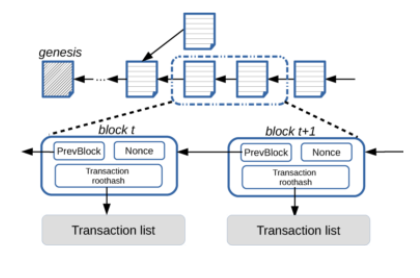
\includegraphics[width=\textwidth]{imgs/blockchain_block_structure.png}
    \caption{Detail view of a block of blockchain}
    \label{fig:Detail view of a block of blockchain}
    \end{figure}

\vspace{1cm}

\textit{SECURITY THEMES FOR CERTIFICATES IN BLOCKCHAIN\\}
Certificates on a blockchain must fulfill certain essential themes namely,
\begin{itemize}
    \item Authentication: identifying whether the user is authentic i.e. the user is registered on the server or the platform
    \item Authorization:process of giving access to specific resources only to authenticated users.
    \item Confidentiality: it's about maintaining secrecy of information between the user and the platform/server.
    \item Ownership: it specifies who owns the data or some resource.
    \item Privacy: it's about maintaining confidentiality about the user details
\end{itemize}

\vspace{1cm}

\textit{LIMITATIONS OF TRADITIONAL VERIFICATION\\}
This section discusses the limitations of the traditional verification system. Existing verification methods do not guarantee records that are not sealed, secured, tamper-proof, and authenticated. five limitations of traditional verification systems which are ownership, availability, dependency on third-party agencies, time consumption and cost. \\
Explanation of each limitation as follows:
\begin{itemize}
    \item Ownership:
The certificate ownership does not automatically appear to the individuals.
\item Availability:
Physical documents may be lost or damaged. Hence, individuals who lose them cannot readily obtain duplicates.
\item Dependency: on third-party agencies
Many organizations depend on third-party verification agencies to contact issuing authorities and verify document authenticity.
\item Time utilization:
The process is time-consuming. The speed of verification depends on the response time of issuing authorities and their location.
\item Cost:
A fee is charged for each verification for the certificate or document.
\end{itemize}


\begin{table}[H]
    \normalsize
    \begin{center}
    \begin{tabular}{|m{4cm}| m{5.5cm}|m{5.5cm}|}
        \hline
        \textbf{PARAMETERS} & \textbf{BLOCKCHAIN} & \textbf{TRADITIONAL VERIFICATION SYSTEM}\\
        \hline
    DOCUMENT PERSPECTIVE & It can avoid the risk of losing or falsifying paper documents. & In this traditional system all the contents are in paper formats.\\
    \hline
    COST-EFFECTIVE & Blockchain helps in transferring the right to control and store the applicant’s personal data to the applicant himself. & Institutions can reliably and responsibly store documents and offer access to the applicants at the request of employers and authorities.\\
    \hline
    PAYMENT METHODS & No payments for intermediate services. & There is a payment for each and every third-party service.\\
    \hline
    DURING TRANSACTION & Transparency of transactions increased. & Transparency of transactions is less.\\
        \hline

        SECURITY & More secure, records are stored in blocks. & Less secure because records are stored in a local database.\\

        \hline

        IMMUTABILITY &
Records to be written and stored permanently, without the possibility of modifications. &
Records are in paper format, so the chance of modifying certificates gets increased.\\

\hline
EFFICIENCY &
More efficient. &
Less efficient. \\

\hline
    \end{tabular}  
    \caption{Comparision of traditional systems and blockchain}
    \label{table-example}
    \end{center}
    \end{table}

\section{IPFS}
\noindent{ IPFS (Inter Planetary File System) is a peer- to peer hypermedia protocol and distributed file system. It has a block storage model with hyperlinks to address the contents forming a Merkle Directed Acyclic Graph. Since IPFS is distributed, it has no single point of failure. IPFS represents a file by the hash on it, instead of representing it by which server it is stored on.
Storing large amounts of data on Ethereum can be very expensive. Content-based addresses that IPFS returns are 46 bytes in size which is a tiny amount considering the size of files. It is cheaper to publish a file on IPFS and store their content-based address on the Ethereum blockchain. \\}

\vspace{1cm}
\textit{HOW IPFS WORKS? }

\begin{itemize}
    \item 
    When you add a file to IPFS, your file is split into smaller chunks, cryptographically hashed, and given a unique fingerprint called a content identifier (CID). This CID acts as a permanent record of your file as it exists at that point in time.
    \item When other nodes look up your file, they ask their peer nodes who's storing the content referenced by the file's CID. When they view or download your file, they cache a copy — and become another provider of your content until their cache is cleared.
    \item A node can pin content in order to keep (and provide) it forever, or discard content it hasn't used in a while to save space. This means each node in the network stores only content it is interested in, plus some indexing information that helps figure out which node is storing what.
    \item If you add a new version of your file to IPFS, its cryptographic hash is different, and so it gets a new CID. This means files stored on IPFS are resistant to tampering and censorship — any changes to a file don't overwrite the original, and common chunks across files can be reused in order to minimize storage costs.
    \item However, this doesn't mean you need to remember a long string of CIDs — IPFS can find the latest version of your file using the IPNS decentralized naming system, and DNSLink can be used to map CIDs to human-readable DNS names.
\end{itemize}

\vspace{1cm}
\textit{Advantages of IPFS}

\begin{itemize}
   \item \underline{Archivists}
Storing archival data using IPFS enables deduplication, clustered persistence, and high performance — empowering you to store the world's information for future generations.

\item \underline{Service providers}
Providing large amounts of data to users? Storing on IPFS could help you slash bandwidth costs thanks to its use of secure, peer-to-peer content delivery.

\item \underline{Researchers}
If you're working with or distributing large datasets, storing that data using IPFS can help speed up performance and unlock decentralized archiving.

\item \underline{Blockchain developers}
IPFS content addressing enables you to store large files off-chain and put immutable, permanent links in transactions — timestamping and securing content without having to put the data itself on-chain.

\item \underline{Content creators}
IPFS empowers creators to build and share on the decentralized web — whether that's delivering content free from intermediary control or minting NFTs that stand the test of time.

\item \underline{Offline users}
High-latency networks cause major obstacles for those with poor internet infrastructure. Peer-to-peer IPFS offers resilient access to data independent of latency or backbone connectivity.

\end{itemize}

\begin{table}[H]
    \normalsize
    \begin{center}
    \begin{tabular}{|m{7cm}| m{7cm}|}
        \hline
        \textbf{HTTP} & \textbf{IPFS} \\
        \hline
        It uses a centralized client server approach &
It uses a decentralized peer to peer approach.\\
        \hline
        Data is requested using the address on which data is hosted &
Data is requested using the cryptographic hash of that data \\
        \hline
        Data cannot be accessed if the server is down or fails or any link gets broken & 
Data is copied to multiple nodes, hence it can be accessed whenever needed.\\
        \hline
        The bandwidth provided is low, as multiple clients request from a single server at the same time. &
        Bandwidth is high, as data is requested from the closest peer who has the copy of that data.\\
        \hline
        One has to set up a hosting server or pay for one, in order to make content publicly available. &
Uploading content on the IPFS network does not require a host server, every node hosts the data on the network.\\
        \hline
        HTTP is well established as an industry standard, this is where HTTP has an upper hand. &
IPFS is relatively newer and is not yet as popular as HTTP.\\
\hline 
HTTP support is inbuilt on almost all machines. &
To run IPFS you need to access it using the HTTP to IPFS portal or manually set up an IPFS node on your machine.\\

\hline
HTTP is used by almost everyone to access the web.	&
Currently, there is a shortage of IPFS nodes due to its low popularity among the laymen.\\
\hline
    \end{tabular}  
    \caption{HTTP v/s IPFS}
    \label{table-example}
    \end{center}
    \end{table}

\section{Ethereum}
\noindent{
    Ethereum is a technology that lets you send cryptocurrency to anyone for a small fee. It also powers applications that everyone can use and no one can take down.\\
It's the world's programmable blockchain.
Ethereum builds on Bitcoin's innovation, with some big differences.\\
Both let you use digital money without payment providers or banks. But Ethereum is programmable, so you can also use it for lots of different digital assets – even Bitcoin!
This also means Ethereum is for more than payments. It's a marketplace of financial services, games and apps that can't steal your data or censor you.}

\section{Smart Contract}
\noindent{A smart contract is a self-executing contract with the terms of the agreement between buyer and seller being directly written into lines of code. The code and the agreements contained therein exist across a distributed, decentralized blockchain network.Smart contracts render transactions traceable, transparent, and irreversible.}